\documentclass{article}
\usepackage[svgnames]{xcolor}
\usepackage[utf8]{inputenc}
\usepackage{pdfpages}
\usepackage{float}
\usepackage{fullpage} % Package to use full page
\usepackage{parskip} % Package to tweak paragraph skipping
\usepackage{tikz} % Package for drawing
\usepackage{amsmath}
\usepackage{hyperref}
\hypersetup{
    colorlinks=true,
    linkcolor=purple,
    filecolor=magenta,      
    urlcolor=pink,
}
\usepackage{amssymb}
\usepackage{bm}
\usepackage{framed}
\usepackage{amsthm}
\usepackage{listings}
\usepackage{biblatex}

\lstset{language=R,
    basicstyle=\small\ttfamily,
    stringstyle=\color{DarkGreen},
    otherkeywords={0,1,2,3,4,5,6,7,8,9},
    morekeywords={TRUE,FALSE},
    deletekeywords={data,frame,length,as,character},
    keywordstyle=\color{blue},
    commentstyle=\color{DarkGreen},
}

\addbibresource{glm-exercises.bib}

\newenvironment{lyxcode}
	{\par\begin{list}{}{
		\setlength{\rightmargin}{\leftmargin}
		\setlength{\listparindent}{0pt}% needed for AMS classes
		\raggedright
		\setlength{\itemsep}{0pt}
		\setlength{\parsep}{0pt}
		\normalfont\ttfamily}%
	 \item[]}
	{\end{list}}


\newcommand\independent{\protect\mathpalette{\protect\independenT}{\perp}}
\def\independenT#1#2{\mathrel{\rlap{$#1#2$}\mkern2mu{#1#2}}}

\newcommand{\E}{\mathrm{E}}
\newcommand{\Var}{\mathrm{Var}}
\newcommand{\Cov}{\mathrm{Cov}}
\newcommand{\Cor}{\mathrm{Cor}}

% vertical line in {bmatrix}
\makeatletter
\renewcommand*\env@matrix[1][*\c@MaxMatrixCols c]{%
 \hskip -\arraycolsep
 \let\@ifnextchar\new@ifnextchar
 \array{#1}}
\makeatother

\title{Exercises in Generalized Linear Models \\ \textbf{Week 42}}
\author{Vinnie Ko, Jonas Moss, and Ørnulf Borgan}
\date{Fall 2020}

\begin{document}
\maketitle
Exercises for the course \href{https://www.uio.no/studier/emner/matnat/math/STK3100/}{STK3100/STK4100: Introduction to Generalized Linear Models} at the University of Oslo, fall 2020. The exercises are from the textbook Alan Agresti: \textit{Foundations of Linear and Generalized Linear Models}. Wiley, 2015. ISBN: 978-1-118-73003-4. The additional exercises are available \href{https://www.uio.no/studier/emner/matnat/math/STK3100/h20/oppgaver.html}{online}. Exercises exclusively nvolving \texttt{R} are not covered.
\section*{Exercise 20}
\subsection*{(a)}

\subsubsection*{(i)}
It's given that $A \sim \mathrm{Bin}(A+C,\pi(1))$. So, the pmf is $f(A) = \binom{A+C}{A}\pi(1)^{A} (1-\pi(1))^{A+C-A}$. Then the log-likelihood is
\begin{align*}
L(\pi(1)) &= \log\binom{A+C}{A} + A\log\pi(1) + C\log(1-\pi(1))
\end{align*}
We find the MLE of $\pi(1)$
\begin{align*}
\frac{\partial L(\pi(1))}{\partial \pi(1)} = \frac{A}{\pi(1)} -\frac{C}{1-\pi(1)} = 0
\end{align*}
So, $\widehat{\pi}(1) = \frac{A}{A+C}$.\\

By repeating the same for $B \sim \mathrm{Bin}(B+D,\pi(1))$, we obtain $\widehat{\pi}(0) = \frac{B}{B+D}$.\\


\subsubsection*{(ii)}
Now we obtain MLE of odds ratio by using the `plug-in principle' of MLE
\begin{align*}
\widehat{\mathrm{OR}} = \frac{\frac{\widehat{\pi}(1)}{1-\widehat{\pi}(1)}}{\frac{\widehat{\pi}(0)}{1-\widehat{\pi}(0)}} = \frac{\widehat{\pi}(1)}{\widehat{\pi}(0)} \cdot \frac{1-\widehat{\pi}(0)}{1-\widehat{\pi}(1)} = \frac{A(B+D)}{B(A+C)}\cdot\frac{D(A+C)}{C(B+D)} = \frac{AD}{BC}.\\
\end{align*}

\vspace{\baselineskip}
\subsection*{(b)}

\subsubsection*{(i)}
This follows directly from the `plug-in principle' of MLE.


\subsubsection*{(ii)}

By CLT, we know that
\begin{align*}
\widehat{\pi}(j) ~\overset{d}{\to}~ N\left(\pi(j), \, \mathcal{I}_{\pi(j)}^{-1}\right)
\end{align*}
where
\begin{align*}
\mathcal{I}_{\pi(j)} = \E\left[-\frac{\partial^{2} L(\pi(j))}{\partial \pi(j)^2}\right] =
\begin{cases}
\E\left[\frac{B}{\pi(0)^{2}} + \frac{D}{(1-\pi(0))^{2}}\right] & \text{if}~ j = 0\\
\\
\E\left[\frac{A}{\pi(1)^{2}} + \frac{C}{(1-\pi(1))^{2}}\right] & \text{if}~ j = 1
\end{cases}.
\end{align*}

\vspace{0.5cm}
\begin{framed}
\textit{Multivariate Delta method}\\

Suppose that
\begin{align*}
\sqrt{n}(\bm{X}_{n} - \bm{\eta}) ~\overset{d}{\to}~ N_{r}\left(\bm{0}, \bm{\Sigma}\right),
\end{align*}
for some $r$-dimensional random vector $\bm{X}_{n}$ depending on $n$. If $S$ is a function $\mathbb{R}^{r} \to \mathbb{R}^{s}$ which is once differentiable at $\bm{\eta}$ and has Jacobian matrix $\dot{\bm{S}}(\bm{\eta})$, then
\begin{align*}
\sqrt{n}\left(S(\bm{X}_{n}) - S(\bm{\eta})\right) ~\overset{d}{\to}~ N_{s}\left(\bm{0},~ \dot{\bm{S}}(\bm{\eta})^{\rm T} \, \bm{\Sigma} \, \dot{\bm{S}}(\bm{\eta})\right),
\end{align*}
provided that $\dot{\bm{S}}(\bm{\eta})^{\rm T} \, \bm{\Sigma} \, \dot{\bm{S}}(\bm{\eta})$ is positive definite.
\end{framed}

Applying delta method with $\theta(j) = \log\left(\frac{\pi(j)}{1-\pi(j)}\right)$ gives
\begin{align*}
\widehat{\theta}(j) ~&\overset{d}{\to}~ N\left(\theta(j), \, \left(\frac{\partial \theta(j)}{\partial \pi(j)}\right)^{2} \mathcal{I}_{\pi(j)}^{-1}\right)\\
&= N\left(\theta(j), \, \left(\mathcal{I}_{\pi(j)}\pi(j)^{2}\left(1-\pi(j)\right)^{2}\right)^{-1}\right).\\
\end{align*}

We can estimate $\left(\mathcal{I}_{\pi(j)}\pi(j)^{2}\left(1-\pi(j)\right)^{2}\right)^{-1}$ by replacing $\pi(j)$ with $\widehat{\pi}(j)$ and $\mathcal{I}_{\pi(j)}$ by $\mathcal{J}_{\pi(j)}$ (observed information).\\

When $j = 0$,
\begin{align*}
\widehat{\Var}\left(\widehat{\theta}(0)\right) &= \left(\mathcal{J}_{\widehat{\pi}(0)}\widehat{\pi}(0)^{2}\left(1-\widehat{\pi}(0)\right)^{2}\right)^{-1}\\
&= \left(\left(\frac{B}{\widehat{\pi}(0)^{2}} + \frac{D}{(1-\widehat{\pi}(0))^{2}}\right)\cdot \widehat{\pi}(0)^{2}\left(1-\widehat{\pi}(0)\right)^{2} \right)^{-1}\\
&= \left(B\left(1-\widehat{\pi}(0)\right)^{2} + D \, \widehat{\pi}(0)^{2}\right)^{-1}\\
&= \left(\frac{BD^{2}}{(B+D)^{2}} + \frac{B^{2}D}{(B+D)^{2}}\right)^{-1}\\
&= \left(\frac{BD}{B+D}\right)^{-1}\\
&= \frac{B+D}{BD}\\
&= \frac{1}{B} + \frac{1}{D}.
\end{align*}

Similarly, when $j = 1$,
\begin{align*}
\widehat{\Var}\left(\widehat{\theta}(1)\right) &= \frac{1}{A} + \frac{1}{C}.
\end{align*}

\vspace{\baselineskip}
\subsection*{(c)}

i)
\begin{align*}
\mathrm{SE}\left(\log\widehat{\mathrm{OR}}\right)^{2} &= \widehat{\Var}\left(\log\widehat{\mathrm{OR}}\right)\\
&= \widehat{\Var}\left(\widehat{\theta}(1) - \widehat{\theta}(0)\right)\\
&= \widehat{\Var}\left(\widehat{\theta}(1)\right) + \widehat{\Var}\left(\widehat{\theta}(0)\right) \tag{$\because A \independent B$}\\
&= \frac{1}{A} + \frac{1}{C} + \frac{1}{B} + \frac{1}{D}\\
&= \frac{1}{A} + \frac{1}{B} + \frac{1}{C} + \frac{1}{D}\\
\end{align*}

\subsubsection*{(ii)}
A $95\%$ confidence interval of $\log\mathrm{OR}$:
\begin{align*}
\log\widehat{\mathrm{OR}} \pm z_{0.975}\cdot\mathrm{SE}\left(\log\widehat{\mathrm{OR}}\right).
\end{align*}
By taking $exp$ on the both side we obtain a $95\%$ confidence interval of $\mathrm{OR}$:
\begin{align*}
\widehat{\mathrm{OR}} \cdot \exp\left[\pm z_{0.975}\cdot\mathrm{SE}\left(\log\widehat{\mathrm{OR}}\right)\right].
\end{align*}

\vspace{\baselineskip}
\subsection*{(d)}
\begin{lstlisting}
> # Enter the data
> diabetes = as.data.frame(matrix(c(377, 17864, 336, 20099), 2, 2))
> rownames(diabetes) = c("diseased","healthy")
> colnames(diabetes) = c("male","female")
> show(diabetes)
          male female
diseased   377    336
healthy  17864  20099
> 
> # Perform chi-square test
> chisq.test(diabetes)

	Pearson's Chi-squared test with Yates' continuity correction

data:  diabetes
X-squared = 9.277, df = 1, p-value = 0.00232
\end{lstlisting}

p-value: $0.00232 < 0.05$. So, we conclude that there is significance difference between the occurrence of diabetes between men and women.


\vspace{\baselineskip}
\subsection*{(e)}
By using the result from c), we obtain the $95\%$ confidence interval of odds ratio for diabetes between men and women.

\begin{lstlisting}
> # Estimated odds ratio
> OR.hat = diabetes[1,1]*diabetes[2,2]/(diabetes[1,2]*diabetes[2,1])
> show(OR.hat)
[1] 1.262402
> # Standard error of log of odds ratio
> std.error = sqrt(sum(1/diabetes))
> 
> # 95% confidence interval of odds ratio
> low.CI = OR.hat*exp(-qnorm(0.975)*std.error)
> upp.CI = OR.hat*exp(qnorm(0.975)*std.error)
> c(low.CI, upp.CI)
[1] 1.088277 1.464387
\end{lstlisting}

Thus, $\widehat{\mathrm{OR}} = 1.2624$ and $95\%$ confidence interval of $\mathrm{OR}$: $[1.0883, \, 1.4644]$.

\vspace{\baselineskip}
\subsection*{(f)}

\subsubsection*{(i)}
$\mathrm{OR} = 1 \iff \pi(0) = \pi(1)$.

\subsubsection*{(ii)}
$H_{0}: \pi(0) = \pi(1)$. and we know $\widehat{\pi}(j) ~\overset{\mathrm{approx}}{\sim}~ N\left(\pi(j), \, \mathcal{I}_{\pi(j)}^{-1}\right)$.\\

Since $\mathrm{OR} = 1 \iff \pi(0) = \pi(1)$, we can check whether 1 is in the $95\%$ confidence interval of OR from e):
\begin{align*}
1 \notin [1.0883, \, 1.4644].
\end{align*}
So, we reject the null hypothesis and conclude that there is significance difference between the occurrence of diabetes between men and women.


\vspace{\baselineskip}
\subsection*{(g)}
If we fit logistic regression with \texttt{sex} as covariate, we have
\begin{align*}
\log\widehat{\mathrm{OR}} = \log\left(\frac{\frac{\widehat{\pi}(1)}{1-\widehat{\pi}(1)}}{\frac{\widehat{\pi}(0)}{1-\widehat{\pi}(0)}}\right) = \log\left(\frac{\widehat{\pi}(1)}{1-\widehat{\pi}(1)}\right) - \log\left(\frac{\widehat{\pi}(0)}{1-\widehat{\pi}(0)}\right)= \widehat{\beta}_{1}.
\end{align*}
We can use this relationship to convert the confidence interval of $\widehat{\beta}_{1}$ into the confidence interval of $\widehat{\mathrm{OR}}$.

\begin{lstlisting}
> # Modify data such that it's suitable for logistic regression
> diabetes.glm.form = data.frame(
+   y = as.numeric(diabetes["diseased",]),
+   n = as.numeric(colSums(diabetes)),
+   sex = c(1,0))
> diabetes.glm.form[,"sex"] = as.factor(diabetes.glm.form[,"sex"])
> head(diabetes.glm.form)
    y     n sex
1 377 18241   1
2 336 20435   0
> 
> # Fit logistic regerssion
> diabetes.model.1 = glm(cbind(y, n - y) ~ sex, 
family = binomial(link = "logit"), 
data = diabetes.glm.form)
> summary(diabetes.model.1)

Call:
glm(formula = cbind(y, n - y) ~ sex, family = binomial(link = "logit"), 
    data = diabetes.glm.form)

Deviance Residuals: 
[1]  0  0

Coefficients:
            Estimate Std. Error z value Pr(>|z|)    
(Intercept) -4.09131    0.05501 -74.376  < 2e-16 ***
sex1         0.23302    0.07573   3.077  0.00209 ** 
---

(Dispersion parameter for binomial family taken to be 1)

    Null deviance:  9.4891e+00  on 1  degrees of freedom
Residual deviance: -2.7651e-12  on 0  degrees of freedom
AIC: 19.389

Number of Fisher Scoring iterations: 2

> 
> 
> # Confidence interval based on logistic regression
> beta.1.hat = summary(diabetes.model.1)$coefficients["sex1","Estimate"]
> std.error.beta.1 = summary(diabetes.model.1)$coefficients["sex1","Std. Error"]
> low.CI = exp(beta.1.hat - qnorm(0.975)*std.error.beta.1)
> upp.CI = exp(beta.1.hat + qnorm(0.975)*std.error.beta.1)
> c(low.CI, upp.CI)
[1] 1.088278 1.464387
\end{lstlisting}

As expected, this matches the confidence interval we obtained from e).\\

\vspace{\baselineskip}
\subsection*{(h)}
Repeat d) - g) with the new data.
\section*{Exercise 4.20}
The pmf of Poisson distribution is
\begin{align*}
f(y) = \frac{\mu^{y}}{y!}e^{-\mu}
\end{align*}
So,
\begin{align*}
L(\bm{y}) &= \log\mu\sum_{i=1}^{n}y_{i} - n\mu -\sum_{i}^{n}\log y_{i}!\\
\frac{\partial L(\bm{y})}{\partial \mu} &= \frac{1}{\mu}\sum_{i=1}^{n}y_{i} -n = -n +\frac{n\overline{y}}{\mu}\\
H &= \frac{\partial^{2} L(\bm{y})}{\partial \mu^{2}} = -\frac{n\overline{y}}{\mu^{2}}\\
\mathcal{J} &= \E\left[-\frac{\partial^{2} L(\bm{Y})}{\partial \mu^{2}}\right] = \frac{n}{\mu^{2}}\E\left[\overline{Y}\right] = \frac{n}{\mu}.
\end{align*}

Fisher scoring gives
\begin{align*}
\mu^{(t+1)} = \mu^{(t)} + \left(\mathcal{J}^{(t)}\right)^{-1}u^{(t)} = \mu^{(t)} + \frac{\mu^{(t)}}{n}\left(-n +\frac{n\overline{y}}{\mu^{(t)}}\right) = \overline{y}.
\end{align*}

Newton-Raphson gives
\begin{align*}
\mu^{(t+1)} = \mu^{(t)} + \left(H^{(t)}\right)^{-1}u^{(t)} = \mu^{(t)} -\frac{\left(\mu^{(t)}\right)^{2}}{n\overline{y}}\left(-n +\frac{n\overline{y}}{\mu^{(t)}}\right) = \mu^{(t)}\left(2 - \frac{\mu^{(t)}}{\overline{y}}\right).
\end{align*}
Note that if $\mu^{(t)} = \overline{y}$, then $\mu^{(t+1)} = \overline{y}$.
\section*{Exercise 5.1}

\subsection*{(a)}

Let $X\mid y\sim N(\mu_{y},\sigma^{2})$, so that $P(x\mid y)=\phi(x;\mu_{y},\sigma)$.
Define $P(Y=1)=p,$ $q=1-p$. Then 
\begin{eqnarray*}
P(Y=1\mid x) & = & P(x\mid Y=1)\frac{P(Y=1)}{P(x)},\\
 & = & \frac{p\phi(x;\mu_{1},\sigma^{2})}{p\phi(x;\mu_{1},\sigma^{2})+q\phi(x;\mu_{0},\sigma^{2})},\\
 & = & \frac{1}{1+\frac{q}{p}\frac{\phi(x;\mu_{0},\sigma^{2})}{\phi(x;\mu_{1},\sigma^{2})}}.
\end{eqnarray*}
Here

\[
\frac{\phi(x;\mu_{0},\sigma^{2})}{\phi(x;\mu_{1},\sigma^{2})}=\exp\left(-\frac{1}{2\sigma^{2}}(\mu_{1}^{2}-2x(\mu_{0}-\mu_{1})-\mu_{0}^{2})\right),
\]
and we obtain

\begin{eqnarray*}
\frac{1}{1+\frac{q}{p}\exp\left(-\frac{1}{2\sigma^{2}}(\mu_{1}^{2}-2x(\mu_{0}-\mu_{1})-\mu_{0}^{2})\right)} & =\\
\frac{1}{1+\frac{q}{p}\exp\left(\beta_{0}+x\frac{(\mu_{1}-\mu_{0})}{2\sigma^{2}}\right)}
\end{eqnarray*}
This equals the inverse logistic function applied to $\beta_{0}=-\frac{1}{2\sigma^{2}}(\mu_{1}^{2}-\mu_{0}^{2})+\log(q/p)$.

\subsection*{(b)}

Let $X\mid y\sim N(\mu_{y},\sigma_{y}^{2})$, so that $P(x\mid y)=\phi(x;\mu_{y},\sigma_{y})$.
Define $P(Y=1)=p,$ $q=1-p$. 

Then 
\begin{eqnarray*}
P(Y=1\mid x) & = & P(x\mid Y=1)\frac{P(Y=1)}{P(x)},\\
 & = & \frac{p\phi(x;\mu_{1},\sigma_{1}^{2})}{p\phi(x;\mu_{1},\sigma_{1}^{2})+q\phi(x;\mu_{0},\sigma_{0}^{2})},\\
 & = & \frac{1}{1+\frac{q}{p}\frac{\phi(x;\mu_{0},\sigma_{0}^{2})}{\phi(x;\mu_{1},\sigma_{1}^{2})}}.
\end{eqnarray*}
Here

\begin{eqnarray*}
\frac{q}{p}\frac{\phi(x;\mu_{0},\sigma^{2})}{\phi(x;\mu_{1},\sigma^{2})} & = & \exp\left(-\frac{(\mu_{1}-x)^{2}}{2\sigma_{1}^{2}}+\frac{(\mu_{0}-x)^{2}}{2\sigma_{0}^{2}}+\log(q/p)\right),\\
 & = & \exp\left(\beta_{0}+\beta_{1}x+\beta_{2}x^{2}\right),
\end{eqnarray*}
for some coefficients $\beta_{0},\beta_{1},\beta_{2}$ depending on
$\mu_{0},\mu_{1},\sigma_{0},\sigma_{1},p,q$.

\subsection*{(c)}

Let $P(x\mid y)=h(x)\exp(x\theta_{y}-b(\theta_{y}))$. Define $P(Y=1)=p,$
$q=1-p$. 

Then 
\begin{eqnarray*}
P(Y=1\mid x) & = & P(x\mid Y=1)\frac{P(Y=1)}{P(x)},\\
 & = & \frac{ph(x)\exp(x\theta_{1}-b(\theta_{1}))}{ph(x)\exp(x\theta_{1}-b(\theta_{1}))+qh(x)\exp(x\theta_{0}-b(\theta_{0}))},\\
 & = & \frac{1}{1+\frac{q}{p}\frac{\exp(x\theta_{1}-b(\theta_{1}))}{\exp(x\theta_{0}-b(\theta_{0}))}}.
\end{eqnarray*}
Now we see that
\[
\frac{q}{p}\frac{\exp(x\theta_{1}-b(\theta_{1}))}{\exp(x\theta_{0}-b(\theta_{0}))}=\exp\left(\beta_{0}+\beta_{1}x\right)
\]
for some coefficients $\beta_{0},\beta_{1},\beta_{2}$ depending on
$\mu_{0},\mu_{1},p,q$. 

\subsection*{(d{*})}

The same result as in $b$ holds for aribtrary exponential dispersion
families as well. 

\subsection*{Comments}

This regression speficiation is in reverse; it assumes that we know
regression of $X$ on $Y$, $X\mid Y\sim\mu_{y}+\sigma_{y}\epsilon$.This
flips causality on its head, and doesn't work well with our usual
practice of conditioning on $X$ when doing regression.
\section*{Exercise 5.2}

According note 1.5 on page 21, Hoaglin's partial effect measure for
$\beta_{j}$ is

\[
e_{i}=\frac{1}{n}\sum_{i=1}^{n}\frac{\partial\hat{\mu}_{i}}{\partial x_{ij}}.
\]
In our case, $\hat{\mu}_{i}=\hat{\pi}_{i}$. Recall that 
\[
\hat{\pi}=\frac{1}{1+\exp\left(-\hat{\beta}^{T}x_{i}\right)}
\]
and we can calculate

\begin{eqnarray*}
e_{j} & = & \frac{1}{n}\sum_{i=1}^{n}\frac{\partial\hat{\pi}_{i}}{\partial x_{ij}}\\
 & = & \frac{1}{n}\sum_{i=1}^{n}\frac{\partial}{\partial x_{ij}}\frac{1}{1+\exp\left(-\hat{\beta}^{T}x_{i}\right)},\\
 & = & \hat{\beta}_{j}\frac{1}{n}\sum_{i=1}^{n}\frac{\exp\left(-\hat{\beta}^{T}x_{i}\right)}{\left(\exp\left(-\hat{\beta}^{T}x_{i}\right)+1\right)^{2}},\\
 & = & \hat{\beta}_{j}\frac{1}{n}\sum_{i=1}^{n}\hat{\pi}_{i}(1-\hat{\pi}_{i}).
\end{eqnarray*}

\section*{Exercise 5.4}
When equation (5.5) holds for $\beta_{0}$, $x_{i,j} = 1$ and we have $\sum_{i=1}^{n} n_{i}y_{i} = \sum_{i=1}^{n} n_{i}\pi_{i}$. By dividing $N = \sum_{i=1}^{n} n_{i}$ on both sides, we obtain $\overline{y} = \frac{1}{N}\sum_{i=1}^{n} n_{i}y_{i} = \frac{1}{N}\sum_{i=1}^{n} n_{i}\pi_{i} = \pi$. So, the estimated overall success probability equals overall sample proportion of successes.

This result doesn't hold for binary GLMs where the link function is not logistic link function.
\section*{Exercise 5.30}

A logistic regression model is

\[
E(y_{i})=\textrm{logit}^{-1}(\beta_{0}+\beta_{1}x_{i}),
\]
where $x_{i}=1$ if the $i$th person is a smoker and $0$ if not,
$y_{i}=1$ if the $i$th person has lung cancer, $0$ if not. You
cannot use this model to draw causal conclusions.

The purpose of using controls is to estimatet the causal effect of
smoking. Using controls as in this exercise is called matching or
matched case-control studies.

In matching, we typically want to estimate the average causal effect
of $X$ on $Y$:

\[
E[Y_{X=1}-Y_{X=0}],
\]
where $Y_{X=1}$ is a \emph{counterfactual}, the outcome that would
have happened to patient $Y$ if he had, in fact, smoked. When using
matching, we pretend that the matched person are the same except for
the single factor we want to study, which is smoking in this case. 

The average causal effect can thus be estimated as

\[
\frac{1}{n}\sum(y_{i}[x=1]-y_{i}[x=0]),
\]
where $y_{i}[x=1]$ and $y_{i}[x=0]$ are matched pairs with different
values on the smoking variable.

For more information on causal inference, see e.g. Causal Inference
in Statistics: A Primer (2016) by Pearl et al.
%\input{exam-exercises/exam-2018-problem-2}
\includepdf[pages = {3,4,5,6} ]{exam-exercises/exam-2018-solution.pdf}

\printbibliography
\end{document}
